Dans ce chapitre, je présente les technologies d'accès distants.
Dans un premier temps, je commence par expliquer les notions des VPN et de tunnel VPN. 
De plus, j'y expose les protocoles de tunneling et de chiffrement.
Par la suite, je détaille les protocoles qui peuvent former des tunnels VPN sécurisés. 
Finalement, je passe en revue les solutions propriétaires et celles des fournisseurs d'accès pour les accès distants.

\section{Virtual Private Network - VPN}
Le terme VPN est un acronyme pour « Virtual Private Network ».
Un VPN est par définition un réseau virtuel qui transfère des données privées en créant un tunnel à travers un réseau public.

Historiquement, les VPN étaient construits sur des lignes louées, mais le coût de ces infrastructures était trop important.
Maintenant, les VPN sont basés sur l'Internet dont l'avantage principal est son faible coût.
Mais en utilisant l'Internet, les données privées deviennent accessibles à tout le monde. 
Il a donc été nécessaire de fournir des protocoles permettant d'assurer la confidentialité et l'intégrité des données à travers le réseau public. 

Un tunnel VPN est monté entre deux passerelles VPN ou entre deux hôtes. 
Les deux équipements sont d'un point de vue logique connectées directement l'une à l'autre. 
Le tunnel permet d'envoyer des données du réseau privé à travers le réseau public.
Il encapsule les données dans un protocole compris par les deux extrémités. 
L'émetteur encapsule les données et le destinataire récupère les données. 
En plus de l'encapsulation des données, les tunnels VPN réalisent du chiffrement. 

\subsection{Les types de VPN}
Il existe deux grands types de VPN : les VPN site-à-site et les VPN client-à-site ou VPN "remote access".

\subsubsection{Les VPN site-à-site} 
Ils sont utilisés pour connecter des sites entre eux. 
Le tunnel est monté entre deux passerelles VPN dont les configurations sont connues. 
Le réseau Internet opère comme une liaison WAN entre les sites. 
Les employées peuvent échanger des informations entre les différents sites comme s'ils sont connectés sur le site distant. 
Dans ce cas-ci, nous utilisons principalement des tunnels VPN IPsec. 

\subsubsection{Les VPN client-à-site} 
Ils sont généralement utilisés par des travailleurs pour accéder aux ressources de l'entreprise depuis des emplacements non fiables.  
L'utilisateur se connecte via son ordinateur ou son smartphone à la passerelle VPN de son entreprise.  
Dans ce cas, la configuration n'est pas connue, car selon la localisation de l'utilisateur, les paramètres de connexion changent.  
Il est souvent nécessaire d'installer sur l'appareil mobile un client VPN. 
Nous utilisons majoritairement des tunnels VPN SSL pour leur simplicité de configuration. 
Bien qu'il soit possible de créer des tunnels de ce type avec IPSec.
L'utilisation de SSL est soumise à controverse depuis la découvert de \textit{Hearthbleed}.

Avant de présenter les protocoles IPSec, SSL et TLS, intéressons-nous au protocole de tunneling.
\subsection{Les protocoles de tunneling de couche 2}
Avant de créer le tunnel, ces protocoles se mettent d'accord sur des paramètres de session, comme le protocole de chiffrement.
Une fois les paramètres acceptés par les deux extrémités, le tunnel est monté.
Les données sont envoyées via ce tunnel entre les deux extrémités.
Il est possible de transmettre des données issues de protocole non-routable à travers le réseau public. 
Les données sont encapsulés dans un autre protocole qui est routable.

Par exemple, le protocole AppleTalk n'est pas supporté par l'Internet, mais grâce au tunnel, nous encapsulons le paquet AppleTalk dans un paquet IP. 
Ce paquet est envoyé sur l'Internet qui va le transmettre au destinataire.
Ce dernier désencapsule le paquet IP et récupère le paquet AppleTalk. 

Il est nécessaire que les deux extrémités du tunnel comprennent le protocole encapsulé.
Sinon, la destination ne saura pas capable de traiter le paquet encapsulé. 

\subsubsection{Point-to-Point Tunneling Protocol - PPTP}
C'est un protocole propriétaire de Microsoft.
Il est implémenté depuis Windows 2000 dans toutes les machines Windows et il existe des clients PPTP pour Linux et OS X.
Sa configuration est simple, mais la sécurité qu'il propose n'est pas exempt de tout reproche.

Ce protocole encapsule des frames PPP\footnote{Point-to-Point Protocol} dans un tunnel IP.
Il fonctionne en quatre phases dont une est optionnelle : Link Establishment Phase, Authentication Phase, Callback Control Phase, Network Control Phase.
\begin{enumerate}
	\item La phase une sert à établir, maintenir et terminer la connexion physique entre les deux hôtes. C'est aussi à ce moment que les protocoles d'authentification sont choisis.
	\item Le client PPTP est authentifié en utilisant le protocole PPP. L'authentification peut se faire en claire ou en utilisant des protocoles comme PAP et CHAP. 
	\item La phase trois est optionnel et elle permet une sécurité accrue. Elle déconnecte le client et le serveur. Ensuite, le serveur rappelle le client. 
	\item La dernière phase sert à négocier et implémenter les protocoles de compression et de chiffrement.
\end{enumerate}
\subsubsection{Layer 2 Tunneling Protocol - L2TP}
Ce protocole a été normalisé en utilisant les avantages des protocoles PPTP et L2F de Cisco\footnote{Layer 2 Forwarding}. 
Mais il ne permet toujours pas la confidentialité du trafic. 
Il est possible de faire de l'authentification et du chiffrement avec les paquets PPP, mais la connexion reste vulnérable au niveau de la couche transport. 
Il est donc intéressant d'associer L2TP avec un autre protocole de sécurité comme IPSec.

PPTP  et L2TP ne possèdent pas un niveau de sécurité élevé pour être utilisé comme tunnel VPN à travers Internet.
Ils sont le plus souvent remplacer par des tunnels IPSec ou SSL, qui possèdent un meilleur niveau de sécurité.
\section{Internet Protocol Security - IPSec}
IPsec est un ensemble de protocole visant à sécuriser les données au niveau de la couche réseau. 
Il est composé de trois protocoles : AH (\textit{Authentication Header}), ESP (\textit{Encapsulating Security Payload}) et IKE (\textit{Internet Key Exchange}).
IKE est utilisé lors de la négociation des paramètres du tunnel VPN. 
Les deux autres protocoles fournissent la sécurité des données en les encapsulant au sein du tunnel VPN. 

\subsection{Les protocoles AH et ESP}
Le protocole AH permet uniquement l'authentification. 
L'authentification se fait à l'aide d'un algorithme MAC \footnote{Message Authentication Code} tel que MD5 ou SHA-1.
Cette algorithme prend en input des éléments de l'en-tête IP et calcule un IVC \footnote{Integrity Check Value}.
L'IVC est ajouté dans l'en-tête AH et ce dernier est ajouté au paquet IP.

Le protocole ESP permet l'authentification et le chiffrement des données.

Un schéma des paquets formés est disponible sur la Fig.\ref{fig:ipsecHead} p.\pageref{fig:ipsecHead}.

\begin{figure}
	\centering
	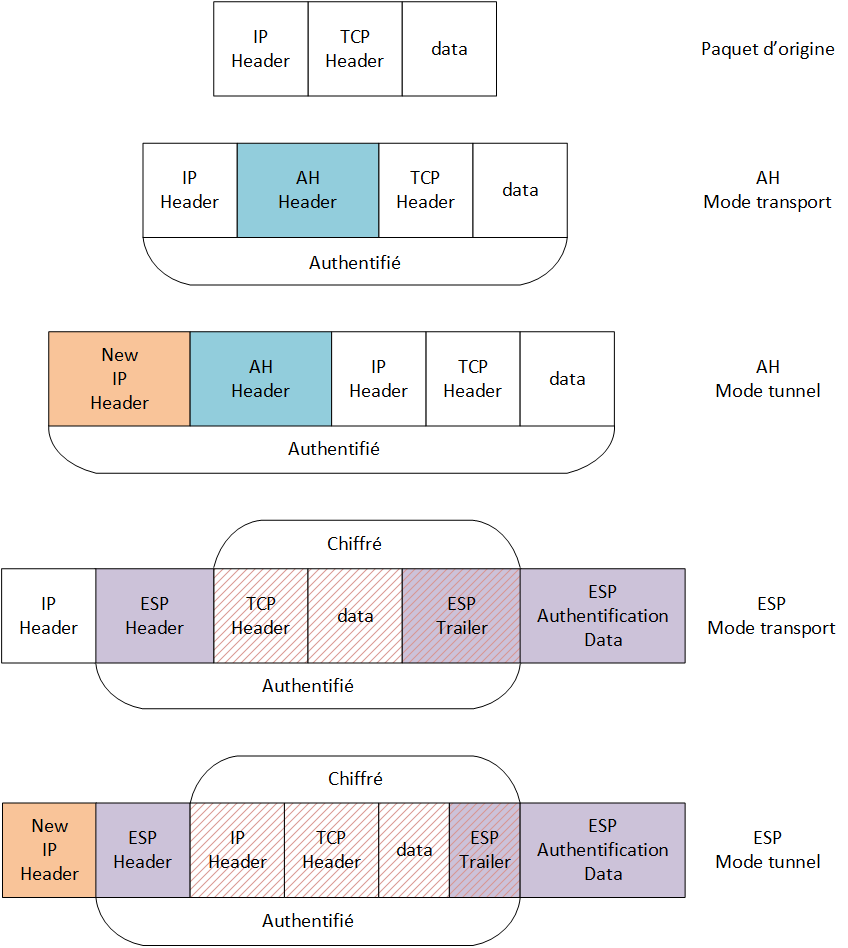
\includegraphics[width=16cm]{techno/IPSec-AH-ESP}
	\caption{Format des paquets IPSec}
	\label{fig:ipsecHead}
\end{figure}

\subsection{Les modes transport et tunnel}
Le mode transport est utilisé pour des connexions bouts-à-bouts entre deux hôtes.

Le mode tunnel est préféré lorsque l'un ou les deux hôtes de la communication sont des passerelles VPN.

\subsection{IPSec et le NAT}
Comme vu précédemment (Fig.\ref{fig:ipsecHead} p.\pageref{fig:ipsecHead}), IPSec protège les en-têtes des paquets IP.
Pour le protocole AH, le moindre changement au niveau des adresses IP provoque une erreur dans l'IVC vu que l'authentification s'applique au paquet entier.
Pour le protocole ESP, l'en-tête ESP est un paquet de la couche réseau. Il ne possède pas d'information sur les ports, qui sont des éléments de la couche transport.
Il n'est pas possible d'associer un port unique pour cette communication.

Pour palier à ces problèmes, une solution est d'encapsuler les paquets IPSec dans un autre paquet.
Ainsi le NAT-T (NAT-Traversal) encapsule les paquets IPSec dans un paquet UDP avec le port 4500 (par défaut).
Ainsi, c'est l'en-tête UDP qui sera modifier lors du transfert entre les deux hôtes et le paquet IPSec ne sera pas modifié.

\subsection{Security association}
Quand nous parlons de monter un tunnel, en réalité, nous synchronisons un état partagé entre les terminaisons du tunnel. 
Cet état partagé se nomme une SA (\textit{security association}) en IPSec. 
Une SA contient l'algorithme de chiffrement utilisé et les clés utilisées, l'algorithme d'authentification, un numéro d'identifiant, le \textit{security parameter index} (SPI), … 
Plus d'autres paramètres qui servent à maintenir les tunnels VPN. 
Les SA peuvent être créées manuellement ou gérées par l'IKE. 
Chaque terminaison possède deux SA, une pour le trafic entrant et une pour le trafic sortant. 
De plus, chaque paire est liée à un protocole. 
Les SA se caractérisent par un triplet formé du SPI, de l'adresse de destination et du protocole. 
Les SA sont stockées dans une SAD (\textit{security association database}). 
Cette SAD est utilisée pour déterminer quel protocole est utilisé pour les paquets sortants et pour fournir les paramètres pour déchiffrer et/ou authentifier les paquets entrants. 
Il est possible de combiner les SA pour créer des tunnels VPN complexe. 

Les SA sont des éléments simples, c'est-à-dire qu'elles traitent tous les paquets de la même manière. 
Pour un réglage plus fin, IPSec utilise des policies. 
Ces policies se basent sur les champs suivants des en-têtes du paquet.
\begin{itemize}
\item L'adresse de destination
\item L'adresse source
\item Le protocole de la couche transport
\item Le port source
\item Le port de destination
\end{itemize}
Elles servent à déterminer quels paquets à émettre sur quel tunnel, à dropper les paquets ne correspondant à aucune des règles décrites dans les policies. 
De la même manière que les SA, les policies sont stockées dans une SPD (\textit{security policy database}). 
Le fonctionnement est similaire, pour chaque paquet entrant ou sortant, le système consulte la SPD pour déterminer les règles à appliquer au paquet. Si une règle est trouvée, le système cherche après la SA correspondante.

\subsection{Le protocole IKE}
IKE a un seul objectif : procéder à des échanges de clé Diffie-Hellman pour sécuriser un tunnel VPN. 
Il négocie le chiffrement, l'authentification nécessaire au tunnel, qui satisfont les policies. 

IKE dérive du \textit{Internet Security Association and Key Management} Protocol (ISAKMP). 
ISAKMP est un framework qui fournit des outils pour la sécurisation des échanges et l'échange de clé. 
De plus, IKE utilise différents mode du protocole OAKLEY.
Il établit une SA en deux phases et il possède cinq modes d'échange, dont trois découlent d'ISAKMP.
Les deux derniers modes ne sont utilisés que lors de la phase deux.

\subsubsection{La phase 1 d'IKE}
La phase 1 crée un canal sécurisé entre les terminaux du tunnel pour déterminer les SA. 
Le canal sécurisé est créé après l'authentification des terminaux. 
Les SA de la phase 1 sont bidirectionnelles, c'est-à-dire qu'une SA sécurise le trafic entrant et sortant. 
Pour l'échange des SA de la phase 1, IKE possède deux modes d'échanges : 
\begin{itemize}
	\item Main mode
	\item Agressive mode
\end{itemize}

Le mode \textit{"main"} d'IKE travaille en trois étapes (voir Fig.\ref{fig:ipsmain} p.\pageref{fig:ipsmain}).
Il est utilisé lorsque les terminaux possèdent des adresses IP statiques. 
\begin{figure}[ht]
\centering
\begin{tikzpicture}
	\draw[-,ultra thick] (0,7) node [above] {Initiator} -- (0,0) ;
	\draw[-,ultra thick] (7,7) node [above] {Responder}-- (7,0);
	\draw[arrow] (0,6) -- (7,6) node [midway,above] {HDR - SA};
	\draw[arrow] (7,5) -- (0,5) node [midway,above] {HDR - SA};
	\draw[arrow] (0,4) -- (7,4) node [midway,above] {HDR - KE - NONCE$_i$};
	\draw[arrow] (7,3) -- (0,3) node [midway,above] {HDR - KE - NONCE$_r$};
	\draw[arrow] (0,2) -- (7,2) node [midway,above] {HDR - ID$_i$ - \textit{AUTH}};
	\draw[arrow] (7,1) -- (0,1) node [midway,above] {HDR - ID$_r$ - \textit{AUTH}};
\end{tikzpicture}
\caption{IPsec : mode "main"}
\label{fig:ipsmain}
\end{figure}
Premièrement, l'initiateur envoie un message contenant une liste des méthodes de sécurisation qu'il utilise. 
Le receveur choisit dans la liste reçue la méthode correspondant à ses policies et envoie sa décision à l'initiateur. 
Ensuite, ce dernier envoie sa clé privée pour créer le secret partagé de l'algorithme de Diffie-Hellman. 
Le receveur fait de même. Ils sont donc capables tous les deux de créer les clés. 
Les clés dépendent des méthodes d'authentification choisies. 
Finalement, l'initiateur envoie son identité et des informations sur l'authentification. 
Ces messages sont chiffrés et masquent donc l'identité des terminaux. 
L'échange se fait en six messages.

À la fin de ce mode, les terminaux sont d'accord sur les algorithmes de chiffrement et de confidentialité des données. 
Ils possèdent également les clés pour les algorithmes sélectionnés. 

Le mode \textit{"agressive"} fait le même travail de façon plus rapide, il n'utilise que trois messages (voir Fig.\ref{fig:ipsagg} p.\pageref{fig:ipsagg}).
Il est utilisé lorsque l'un des deux terminaux de la connexion possède une adresse IP dynamique.
\begin{figure}[ht]
\centering
\begin{tikzpicture}
	\draw[-,ultra thick] (0,4) node [above] {Initiator} -- (0,0) ;
	\draw[-,ultra thick] (8,4) node [above] {Responder}-- (8,0);
	\draw[arrow] (0,3) -- (8,3) node [midway,above] {HDR - SA - KE - NONCE$_i$ - ID$_i$};
	\draw[arrow] (8,2) -- (0,2) node [midway,above] {HDR - SA - KE - NONCE$_r$ - ID$_r$ - \textit{AUTH}};
	\draw[arrow] (0,1) -- (8,1) node [midway,above] {HDR - \textit{AUTH}};
\end{tikzpicture}
\caption{IPsec : mode "agressive"}
\label{fig:ipsagg}
\end{figure} 
Lors du premier envoi, l'initiateur émet la liste des méthodes de sécurisation, son identité et sa clé. 
Le receveur répond par son choix de sécurisation, sa clé, son identité et ses identifiants. 
Finalement l'initiateur s'authentifie auprès du receveur. 
Ce dernier message peut être chiffré.

Pour l'authentification d'un terminal, il existe trois méthodes : 
\begin{itemize}
	\item Kerberos
	\item Certificats	
	\item Public Key Infrastructure (PKI)
\end{itemize}

\paragraph{Kerberos}
Kerberos est un protocole réseau d'authentification par clé chiffré.
Il fournit une forte authentification à condition que tous les services utilisent Kerberos.
Il a été conçue par le MIT\footnote{Massachusetts Institute of Technology} à la fin des années 80.
Actuellement, il est recommandé d'utiliser la version 5, qui corrige des bugs critiques de la version 4.
Kerberos est disponible sur la plupart des systèmes d'exploitation actuels.
Une version gratuite est disponible sur le site du MIT, et il existe des versions commerciales.

Pour qu'un hôte puisse se connecter à un service, le système vérifie son identité, et le cas échéant accepte ou refuse la connexion.
Ce système repose sur deux serveurs sécurisés, un serveur d'authentification (AS\footnote{Authentication Server}) et un serveur d'octroi de ticket (TGS\footnote{Ticket-Granting Server}).
Ils forment dans la terminologie Kerberos un centre de distribution de ticket ou KDC\footnote{Key Distribution Center} en anglais.
De plus, Kerberos utilise des clés chiffrées pour toutes les communications.

\paragraph{Certificat}
Un certificat n'est rien de plus qu'une clé publique accompagnée d'un identifiant dont l'ensemble des informations sont signées par un tiers de confiance.
Ce tiers est ce que l'on appelle une autorité certificative (CA). 
Elle est reconnue au niveau mondiale.
Un utilisateur envoie sa clé publique au CA et reçoit en retour, après vérification, son certificat signé par la CA.

\paragraph{PKI}
Une PKI est un ensemble de composants et de processus informatiques, humains et techniques dont le but est de gérer la distribution et la vie des certificats.

\subsubsection{La phase 2 d'IKE}
Une fois la SA établie, les terminaux peuvent l'utiliser pour négocier les SA de phase 2. 
La phase 2 est un échange en Quick mode. 
L'échange se fait en trois messages. 
Lors de l'échange, il est possible de négocier plusieurs SA en même temps. 
\section{Secure sockets layer - SSL}
Netscape a lancé SSL 1 en 1994, dans le but de sécuriser des transactions réalisées avec leur navigateur. 
Dans la même année, SSL 2 était déjà en route. 
Mais le protocole montrait déjà des problèmes de sécurité.
Fin 1995, SSL 3 était lancé. 
Il s'agissait d'une version complètement récrite de SSL, qui introduisait de nouvelles fonctionnalités issues de PCT\footnote{Microsoft's \textit{Private Communications Technology}}.
Bien que les machines actuelles intègrent SSL 3, elles essaient d'abord de négocier une connexion en SSL 2.

Dans un effort de standardisation de SSL, l'IETF a lancé le protocole TLS\footnote{Transport Layer Security}.
Il se base principalement sur SSL 3 bien qu'il ne soit pas compatible avec ce dernier.

SSL utilise des suites de chiffrement. Ces suites se composent de trois fonctions de chiffrement : la méthode d'échange de clé, l'algorithme de chiffrement et une méthode de hachage. 
Il existe un large ensemble de suite, les client ont donc un mécanisme pour signaler les suites qu'ils gèrent et qu'ils utilisent. 

OpenSSL est l'implémentation la plus courante de SSL. 
Cette implémentation possède un interface en ligne de commande, qui permet de générer des clés RSA, signer des certificats, calculer des valeurs de hash, ...

\subsection{Le protocole SSL}
SSL est un protocole de la couche transport, il utilise donc les protocoles de cette couche pour le transfert des données. 
Pour éviter des problèmes lors de la transmission des données, SSL utilise le protocole TCP.

De manière analogue à TCP, une session SSL se divise en trois phase (voir Fig.\ref{fig:ssl} p.\pageref{fig:ssl}) : 
\begin{enumerate}
	\item \'Etablissement de la connexion
	\item Transfert des données
	\item Clôture de la connexion.
\end{enumerate}
\begin{figure}[ht]
\centering
\begin{tikzpicture}
	\draw[-,ultra thick] (0,10.8) node [above] {Client} -- (0,0) ;
	\draw[-,ultra thick] (6,10.8) node [above] {Serveur}-- (6,0);
	\draw[arrow] (0,10) -- (6,10) node [midway,above] {Handshake : ClientHello};
	\draw[arrow] (6,9) -- (0,9) node [midway,above] {Handshake : ServerHello};
	\draw[arrow] (6,8.4) -- (0,8.4) node [midway,above] {Handshake : Certificate};
	\draw[arrow] (6,7.8) -- (0,7.8) node [sloped, midway,above] {Handshake : ServerHelloDone};
	\draw[arrow] (0,6.8) -- (6,6.8) node [midway,above] {Handshake : KeyExchange};
	\draw[arrow] (0,6.2) -- (6,6.2) node [midway,above] {ChangeCipherSpec};
	\draw[arrow] (0,5.6) -- (6,5.6) node [midway,above] {Handshake : Finished};
	\draw[arrow] (6,4.6) -- (0,4.6) node [midway,above] {ChangeCipherSpec};
	\draw[arrow] (6,4) -- (0,4) node [midway,above] {Handshake : Finished};
	\draw[arrow] (0,2.6) -- (6,2.6);
	\draw[arrow] (6,2) -- (0,2) node [midway,above] {Application Data};
	\draw[arrow] (0,0.8) -- (6,0.8);
	\draw[arrow] (6,0.2) -- (0,0.2) node [midway,above] {Alert Close Notify};
\end{tikzpicture}
\caption{Session SSL}
\label{fig:ssl}
\end{figure}
La session commence par le \textit{triple handshake}. 
Le client envoie un message ClientHello, qui indique la version de SSL supportée, la liste des suites de chiffrement et les algorithmes de compression. 
La version de SSL est signalée par deux champs dans l'en-tête : version mineur et version majeure. 
SSL3 a une version majeure de 3 et une version mineure de 0, et TLS a un version majeure de 3 et une version mineure de 1. 

Le serveur répond par trois messages.
\begin{enumerate}
	\item Le message \textit{ServerHello} indique au client la suite de chiffrement et l'algorithme de compression à utiliser.
	\item Le certificat du serveur permet au client de vérifier l'identité du serveur et contient la clé publique du serveur. Cette clé va servir à générer les différents clés pour la session.
	\item Le message \textit{ServerHelloDone} précise la fin de la séquence \textit{Hello}.
\end{enumerate}
Suite à ces trois messages, le client donne au serveur des inputs pour la génération des clés (\textit{ClientKeyExchange}), signal au serveur qu'il utilise les nouvelles clés pour le chiffrement et l'authentification (\textit{ChangeCipherSpec}) et qu'il a fini le handshake (\textit{Finished}).
 Le serveur répond avec son message \textit{ChangeCipherSpec} et son \textit{Finished}.
 
 Le client et le serveur sont capables de s'échanger des données de façon sécurisé. 
 
 Finalement, la session est clôturée.
\section{Secure Shell - SSH}
SSH a pour objectif de créer une connexion sécurisée.
De la même manière que SSL, SSH est un protocole de la couche applicative et utilise TCP.
Par contre les applications ne doivent pas forcément intégrer SSH pour être utilisées via SSH.

SSH est principalement utilisé pour remplacer \texttt{telnet}, mais il est également possible de faire du VPN.
En effet, SSH fournit de l'authentification et du chiffrement pour les communications entres les machines.

Les tunnels VPN SSH sont peu utilisés, car ils manquent de performance.
Mais ils sont simple à mettre en place.
\section{Secure Socket Tunneling Protocol - SSTP}
SSTP est utilisé pour transporter du trafic PPP/L2TP via du SSL3.
Son avantage réside dans le fait qu'il peut passer à travers les NAT, les proxys et les firewalls. 
\section{HTTP over TLS/SSL - HTTPS}
Il s'agit rien de plus qu'une connexion HTTP chiffrée par SSL ou TLS.
Il fournit une authentification pour les serveurs Web et un chiffrement bidirectionnel pour les communications entre le navigateur Web et le serveur Web.

La confiance envers un site Web est liée à un certificat. 
Ce dernier doit provenir d'une autorité certificative reconnue au niveau mondiale. 
\section{Propriétaires}

\section{Fournisseurs d'accès}
